\section{Task Analysis}
\label{sec:task}
Identify the analysis goals and the corresponding visualization tasks is the first yet significant step in designing a useful tool. In this section, we examine how domain experts normally approach the task of analyzing a model (i.e., assess its strength and weakness) and identify where and how an interactive visualization system can aid in such a process.
Then, we reify the multitude discussion with domain experts into concrete goals, from which we identify the visualization tasks that guide the design and implementation of the proposed tool.

During our long-term collaboration with NLP experts, we have conducted extensive interview and discussion on the common approach employed by research for assessing the behavior of a model.%
The prediction accuracy has its place as an objective evaluation metric to measure the overall effectiveness of the model, however, the accuracy number alone does not provide the full story. 
For example, the model may produce correct predictions for the ``wrong'' reasons (e.g., pickup unintended pattern in the training data that can not be generalized in real word scenarios).
%
As a result, beside using standard metrics, the domain experts often rely on exploration centric approach to 
conduct error analysis and obtain intuition.

There is little one can learn when everything is working as expect, therefore, observing how model make mistakes under various scenarios is at the center of such a process. 
The experts often start with simple failure examples, and then make minor perturbations (replace a word or phrase) to the input and observe the change in the prediction. This exercise help isolate where in the input is likely contributed to the failures. For many NLP models, the attention information (see Section~\ref{sec:attention}) is essential to infer the mechanism of the model. The expert can print out the attention values or generate plots to visualize the alignment between sentences or compare attentions. As the experts explore more variation of similar examples, combined with their domain knowledge, he / she may develop hypotheses about the cause of failures, or ask additional questions, which lead to further experimentation.
%
Since such a process is highly exploratory, get responsive answers to the domain experts' query is essential to maintain the flow of reasoning.

The requirement for such analysis meshed nicely with the benefit of interactive visual exploration. 
Therefore, adopting an visualization system that could provide visual representation of various model information should yield immediate benefits.
%
Moreover, by introducing new visual encoding and summarization, we can drastically expand the ways how domain experts interact with the model, enable exploration options that is not possible before either due to tedious manual operation or lack of communication channels.

Through many discussions and iterations with NLP experts, we solidify the analysis goals as the the following.
%Study the effect of perturbation of input to the prediction.
Firstly, understanding how perturbation (e.g., replacing words) of the input affect the prediction is the curial part of error analysis. It not only measures the prediction sensitivity, but also help reveal the potential source of the errors in the input (\textbf{G1}).
%Understand how attention affect the prediction.
Secondly, study the role and mechanism of attention by examine how variation in the input affect the attention, and how changes in attention affect prediction (\textbf{G1}).
%Study the relationship between model stages (encoder, attention, classifier) and the prediction
So far, we focus on how changes in earlier stage of the model affect later stages or final prediction.
%
However, what if the current prediction is wrong, how can we apply minimal update to the model to produce correct prediction and how would that affect attention.
Thirdly, examine the change of prediction lead to what type of change in each stages and it effects on attention (\textbf{G3}).
%
Based on the NLP analysis goals, we identify the visualization tasks to achieve these goals.

\begin{itemize}
\item \textbf{T1} Visualize the \emph{input}, \emph{attention}, \emph{prediction} of the model.
\item \textbf{T2} Automate the perturbation of the input, explore the perturbation result.
\item \textbf{T3} Customize the \emph{attention} for studying the relationship between attention and prediction
\item \textbf{T4} Visualize the changes in the model stages with respect to prediction change driven model update \shusen{does not make sense}
\end{itemize}


%interrupted when they can not easily receive the answers to their immediate queries. 

% examining examples (e.g, what are the mistakes made by the model), and conduct experiments (e.g., perturb the input and observe the changes), formulate hypothesis (e.g, what are the potential causes for the failure).
%ultimate forms intuition about the strength or the weakness of a given model. 
% , then additional examples or variation of existing examples are bring in to rejected or confirm the hypotheses. And new questions or hypothesis may arise.
%Such an analysis is iterative in nature and guided by domain knowledge and hypotheses based on the architecture. As they ask more questions and experiment 
%experiment with model iterate their understanding of the model behavior, ultimate forms intuition about the strength or the weakness of a given model. 
%and come up hypothesis about the potential cause for the failure. 



%\begin{figure}[htbp]
%\centering
%\vspace{-2mm}
% 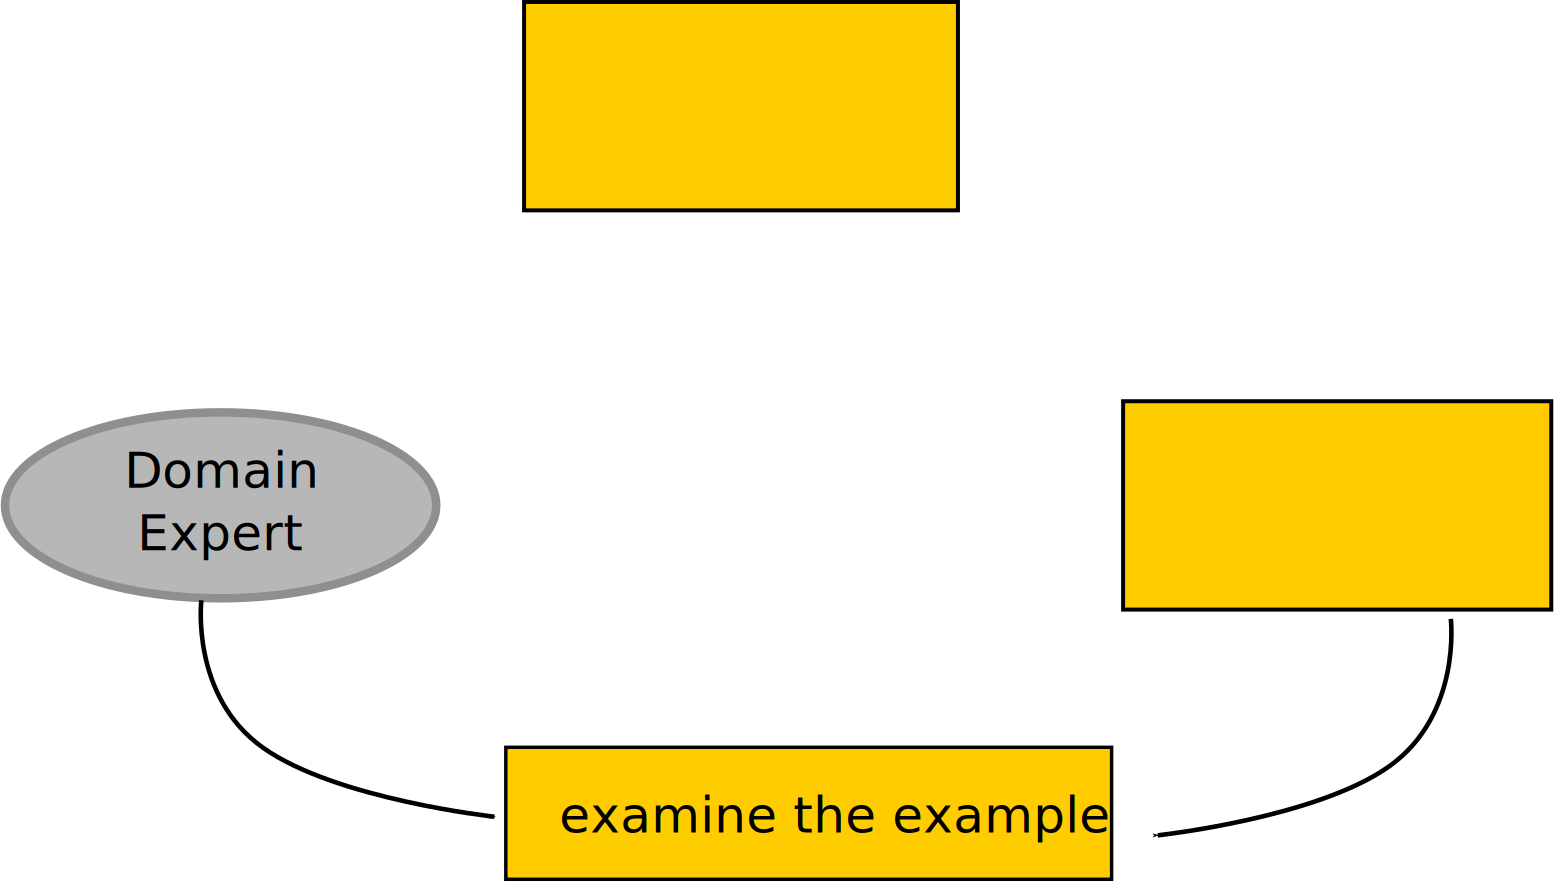
\includegraphics[width=1.0\linewidth]{errorAnalysis}
% \caption{How domain experts conduct error analysis on the model.}
%\label{fig:modelPipeline}
%\end{figure}

